%==========================オプションおよび文書クラスの設定==========================
%"autodetect-engine"-どのエンジンでもコンパイル可能にするオプション
%"dvipdfmx-if-dvi"-必要な場合のみdvipdfmx経由のpdf化をするオプション(LuaTeXやXeTeXはPDFに直接変換するため)
%"ja=standard"-日本語文書の標準設定を利用するオプション
%"bxjs…"-どのエンジンでも利用可能なドキュメントクラス
%--以下のいずれかを選択--
\documentclass[autodetect-engine,dvipdfmx-if-dvi,ja=standard,a4paper,11pt]{bxjsarticle} %章の無いレポート
%\documentclass[autodetect-engine,dvipdfmx-if-dvi,ja=standard,a4paper,10pt]{bxjsslide} %スライド
%\documentclass[autodetect-engine,dvipdfmx-if-dvi,ja=standard,a4paper,10pt]{bxjsbook} %書籍
%\documentclass[autodetect-engine,dvipdfmx-if-dvi,ja=standard,a4paper,10pt]{bxjsreport} %章のある論文やレポート

%==============================プリアンブルの設定==============================
\title{春期課題} %タイトル
\author{新B4 福田真悟} %著者名
\date{2020.3.3}%日付 %日付下の余白をN[mm]減らす

%///////////////////////////////////////////////////////////////////////////////////////////////////////////
%////////////////////////////////////パッケージの読込み及び設定の書換え//////////////////////////////////////
%///////////////////////////////////////////////////////////////////////////////////////////////////////////
\usepackage{graphicx} %図の挿入に関するパッケージ
\usepackage{float} %[H]で図の位置を固定する機能をONにするパッケージ
\usepackage{subcaption} %サブキャプションに関するパッケージ
\captionsetup{labelsep=space} %サブキャプション後の":"を非表示にする
\usepackage{enumerate} %{enumerate}[]の,[]の中の通りの箇条書きにすることができるパッケージ
\usepackage{amsmath} %数式に関するパッケージ
\usepackage{mathtools} %数式に関するパッケージ
\usepackage{bm} %ベクトル表示のコマンドを追加するパッケージ
\usepackage{comment} %複数行のコメントアウトを可能にするパッケージ
\usepackage{ascmac} %枠に関するパッケージ
\usepackage{tabularx} %表に関するパッケージ
\setpagelayout{top=10truemm,bottom=15truemm,left=15truemm,right=15truemm}  %余白に関する設定の書換え(bxjs…クラスではgeometryパッケージは使用不可)
\graphicspath{{../figures/}} %図を挿入する際に.texファイルの上の階層にあるfiguresというフォルダを参照可能にする
\usepackage{url}

%余白に関する設定の書換え(bxjs…クラスではgeometryパッケージは使用不可)
\belowcaptionskip=-0pt %キャプション下の余白をN[pt]減らす
\graphicspath{{../figures/}} %図を挿入する際に.texファイルの上の階層にあるfiguresというフォルダを参照可能にする

%使用記号の追加
\newcommand{\divergence}{\mathrm{div}\,}  %ダイバー
\newcommand{\grad}{\mathrm{grad}\,}  %グラディエント
\newcommand{\rot}{\mathrm{rot}\,}  %ローテーション

%\pagestyle{myheadings} %myheading文字列 emptyページ番号なし plainフッダーに
%\markright{\footnotesize 2月28日(金)15:00~ 顔合わせ}%全ページ共通への挿入
%================================以下本文================================
\begin{document}
\maketitle %設定したタイトルの挿入
\section{\normalsize"Lorenz 方程式","Rossler 方程式","ホワイトガウスノイズ","Logistic 写像"
,"順列エントロピー","相互情報量","複雑ネットワーク"について書籍やインターネットで調べる
}%sectionの前に*をつけると数字の振り分けが消える不思議


\begin{itemize}
\item Lorenz 方程式\\%%%%%%%%%%%%%%%%%%%%%%%%%%%%%%%%%%%%%%%%%%%%%%%%%%%%%%%%%%%%%%%%%%%%%%%%%%%%%%%%%%%%%
 カオス的なふるまいを示す非線形微分方程式の1つで
\begin{equation}
\frac{dx}{dt}=-px+py
\end{equation}
\begin{equation}
\frac{dy}{dt}=-xz+rx-y
\end{equation}
\begin{equation}
\frac{dz}{dt}=xy-bz
\end{equation}
で表現される \cite{lo} .変数は$(x,y,z,t)$,定数は$(p,r,b)$である.初期値鋭敏性から初期値によって,それ以降の結果が大きく変化してしまう.そのため初期値の精度には無限大の精度が必要となり,予測が事実上不可能となっている.

\begin{figure}[H]%[h]は記述したところ。[t]はそのページの上端。[t]はそのページの下端、[p]はページいっぱい
\begin{center}

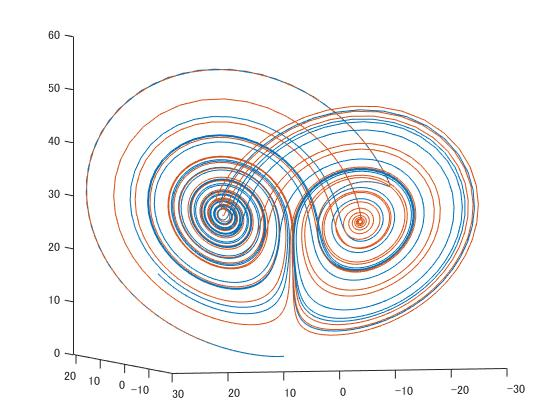
\includegraphics[width=.4\textwidth]{Lorenz_result.jpg}
\end{center}
\caption{Lorenz方程式の誤差の増幅}%図名
\label{fig:lorenz}
\end{figure}

図 \ref{fig:lorenz}は初期値の1つを0.1変化させたときの解の変化である.\\

\item Rossler 方程式\\%%%%%%%%%%%%%%%%%%%%%%%%%%%%%%%%%%%%%%%%%%%%%%%%%%%%%%%%%%%%%%%%%%%%%%%%%%%%%%%%%%%%%
 カオス的なふるまいを示す非線形微分方程式の1つで
\begin{equation}
\frac{dx}{dt}=-y-z
\end{equation}
\begin{equation}
\frac{dy}{dt}=x+ay
\end{equation}
\begin{equation}
\frac{dz}{dt}=b+xz-cz
\end{equation}
で表現される \cite{re} .変数は$(x,y,z,t)$,定数は$(a,b,c)$である.Lorenz方程式と違い,カオスの挙動を把握するために単純化された方程式であり,実際の物理モデルがベースではない.Lorenz方程式と同様に初期値鋭敏性から初期値によって,それ以降の結果が大きく変化してしまう.そのため初期値の精度には無限大の精度が必要となり,予測が事実上不可能となっている.

\begin{figure}[H]%[h]は記述したところ。[t]はそのページの上端。[t]はそのページの下端、[p]はページいっぱい
\begin{center}
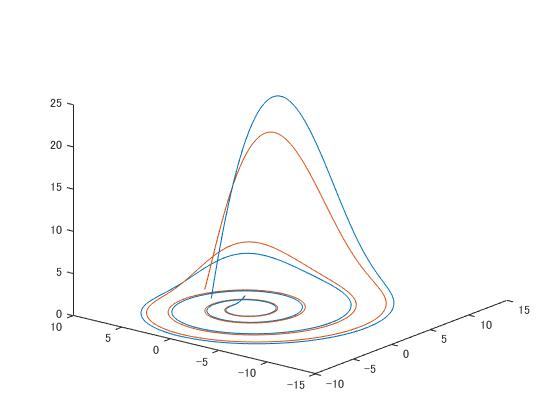
\includegraphics[width=.4\textwidth]{Rossler_result.jpg}
\end{center}
\caption{Rossler方程式の誤差の増幅}%図名
\label{fig:rossler}
\end{figure}

図 \ref{fig:rossler}は初期値の1つを0.1変化させたときの解の変化である.\\


\item ホワイトガウスノイズ\\%%%%%%%%%%%%%%%%%%%%%%%%%%%%%%%%%%%%%%%%%%%%%%%%%%%%%%%%%%%%%%%%%%%%%%%%%%%%%%%%%%%%%
 自然界などのランダム過程の効果をモデル化したもの.ホワイトは周波数帯域が均一であることを示している.光の白色から由来している.ガウスは自然界のものはガウス分布に従うという仮定をもとにノイズもガウス分布となっていることを示している.波形の周波数は均一にすべての周波数で,波形の振幅はガウス分布に従う振幅となっていると仮定したノイズ.モデル化されたノイズのためホワイトガウスノイズサンプルの生成を行う関数が作られている \cite{wgn} .\\

\item Logistic 写像\\%%%%%%%%%%%%%%%%%%%%%%%%%%%%%%%%%%%%%%%%%%%%%%%%%%%%%%%%%%%%%%%%%%%%%%%%%%%%%%%%%%%%%
 Logistic方程式を離散化することで得られる漸化式である.
\begin{equation}
x_{n+1}=ax_{n}(1-x_{n})
\end{equation}
で表現される \cite{logi} .定数$a$によって,値の変化が大きく変わる.$a$が十分に小さいときは0に収束し,値が大きくなるにつれて,収束値が大きくなり,周期的な振動を示し,最終的にカオス的な挙動を示す.$a$ごとの$x$の値の変化を下記に示す.

\begin{figure}[H]%[h]は記述したところ。[t]はそのページの上端。[t]はそのページの下端、[p]はページいっぱい
\begin{center}
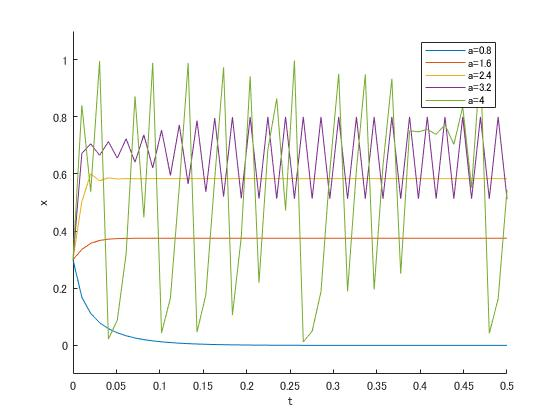
\includegraphics[width=.4\textwidth]{Logistic_result.jpg}
\end{center}
\caption{$a$の変化によるLogistic写像の値の変化}%図名
\label{fig:logstic}
\end{figure}


\item 順列エントロピー\\%%%%%%%%%%%%%%%%%%%%%%%%%%%%%%%%%%%%%%%%%%%%%%%%%%%%%%%%%%%%%%%%%%%%%%%%%%%%%%%%%%%%%
 時系列の乱雑さを定量評価する指標であり,時系列の値ではなく,大小を比較する手法である.長さが$L$の時系列に対して遅れ時間$\tau$の間隔があるデータ$D$個を$D$次元の遅れ時間座標${\bf X}_{\sl j}{\sl=\{ x_j,x_{j+\tau},\cdots ,x_{j+(D-1)\tau} \}} $とし,この座標を考える.ただし,$j=1,2,\cdots,L-(D-1)\tau$とする.この$D$次元の座標のそれぞれの値の大小をパターン化すると$D!$個のランクオーダーパターンに分類される.あるランクオーダーパターン$\pi_i$の相対度数$p(\pi_i)$は,
\begin{equation}
p(\pi_i)=\dfrac{\displaystyle\sum^N_{j=1}\chi_i(X_j)}{L-(D-1)\tau}
\end{equation}
$\chi_i(X_j)$は指示関数であり,
\begin{eqnarray}
\chi_i(X_j)=\left\{ \begin{array}{ll}
1 &  (\pi_j=\pi_i) \\
0 & (\pi_j\neq\pi_i) \\
\end{array} \right.
\end{eqnarray}
となる.そしてこの相対度数の情報エントロピー(Shannonエントロピー)で計算したものが順列エントロピーである.さらに定量的に様々な時系列を比較するために正規化を行ったものを順列エントロピーと定義する.その式を下記に示す.
\begin{equation}
H_p=\dfrac{-\displaystyle\sum_{i=1}^{D!} p(\pi_i) \log_2 p(\pi_i)}{\log_2 D!}
\end{equation}
\\

\item 相互情報量\\%%%%%%%%%%%%%%%%%%%%%%%%%%%%%%%%%%%%%%%%%%%%%%%%%%%%%%%%%%%%%%%%%%%%%%%%%%%%%%%%%%%%%
 2つの情報源の依存度を表した値である.一方の情報をもっているとき,他方の情報を得たらどの程度の不確かさ(情報)2つの情報源が減少するのかを示している.$X,Y$からそれぞれから情報$x,y$を得られる確率を$P_X(x),P_Y(y)$とし,同時に得られる確率を$P_{X,Y}(x,y)$とすると,相互情報量の式は,
\begin{equation}
H_p=\displaystyle\sum_{x\in X}\displaystyle\sum_{y\in Y} P_{X,Y}(x,y) \log_2 \dfrac{P_{X,Y}(x,y)}{P_X(x)P_Y(y)}
\end{equation}
となる \cite{mutual} .
 
\\

\item 複雑ネットワーク\\%%%%%%%%%%%%%%%%%%%%%%%%%%%%%%%%%%%%%%%%%%%%%%%%%%%%%%%%%%%%%%%%%%%%%%%%%%%%%%%%%%%%%
ノード(点)間をリンク(線)で結んで構成されているものをネットワークという.その中で「スケールフリー性」,「スモールワールド性」などの特徴をもつものを複雑ネットワークという.
\\

\end{itemize}


\section{\normalsize相互情報量とLorenz 方程式に関するMATLAB ファイル(mutual.m) を実行し,図を出力する}
出力された結果を下記に示す.

\begin{figure}[H]%[h]は記述したところ。[t]はそのページの上端。[t]はそのページの下端、[p]はページいっぱい
\begin{center}
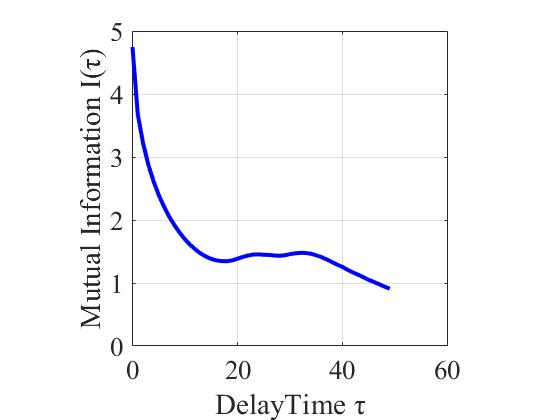
\includegraphics[width=.4\textwidth]{kadai2_rusult.jpg}
\end{center}
\caption{課題2の出力結果}%図名
\label{fig:kadai2}
\end{figure}


\section{\normalsizeホワイトガウスノイズと順列エントロピーに関するMATLABファイル(B4kadai\_2020.m)を実行し,図を出力し考察を加える.}
まず出力された結果を下記に示す.このときのホワイトガウスノイズの生成数は$10000$個で次元数は$5$,遅れ時間は$1$である.

\begin{figure}[H]%[h]は記述したところ。[t]はそのページの上端。[t]はそのページの下端、[p]はページいっぱい
\begin{center}
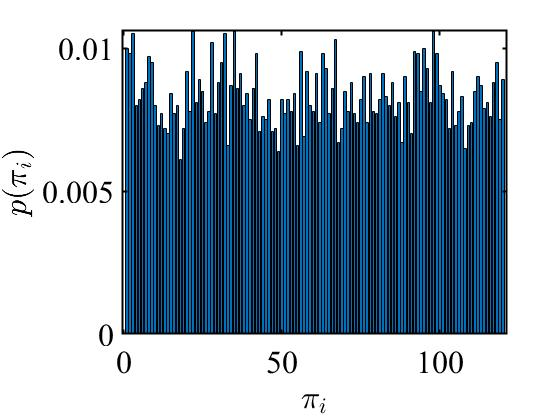
\includegraphics[width=.4\textwidth]{kadai3_rusult.jpg}
\end{center}
\caption{課題3の出力結果(生成数は$10000$個で次元数は$5$,遅れ時間は$1$)}%図名
\label{fig:kadai3}
\end{figure}

この結果からホワイトガウスノイズのランクオーダーパターンにはバラつきがあることがわかる.しかし,ホワイトガウスノイズは周波数帯域が均一のため理論的には,ランクオーダーパターンも均一になると考えられる.今回のシミュレーションでは,次元数$5$($5!=120$個のパターン)に対して,ノイズの生成数が$10000$となっているので平坦に見えるにはデータ数が少ない.実際に$p(\pi_i)$の平均値は約$0.083(=1/120)$となっており,各ランクオーダーパターンの相対度数のヒストグラムを制作すると約$0.083(=1/120)$を中心にガウス分布に近いものとなっている.ノイズの生成を増やせば,各ランクオーダーパターンの相対度数は均一に近づいていくと考えられる.下記にノイズの生成数が$100000$とノイズの生成数が$1000000$に増やしたときの出力結果を示す.


\begin{figure}[H]%[h]は記述したところ。[t]はそのページの上端。[t]はそのページの下端、[p]はページいっぱい
\begin{center}
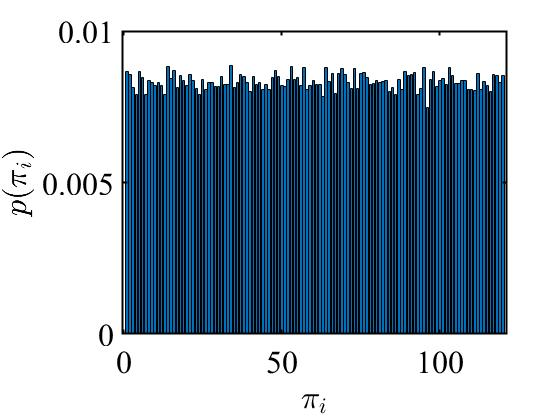
\includegraphics[width=.4\textwidth]{kadai3_result2.jpg}
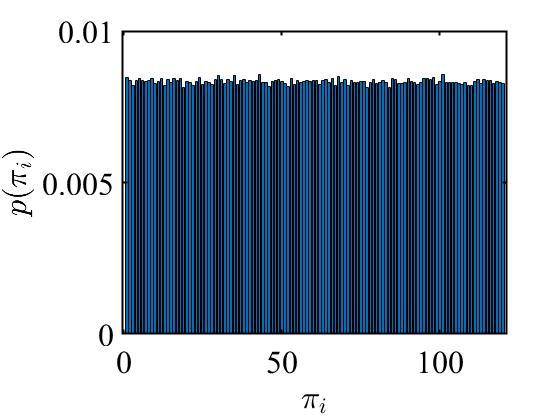
\includegraphics[width=.4\textwidth]{kadai3_result3.jpg}
\end{center}
\caption{課題3の出力結果(左が生成数は$100000$,右が生成数は$1000000$)}%図名
\label{fig:kadai3_2}
\end{figure}

この結果からデータ数を増やすことでバラつきが小さくなることがわかった.また,ノイズの生成数が$100000$のときのヒストグラムも下記に示す.

\begin{figure}[H]%[h]は記述したところ。[t]はそのページの上端。[t]はそのページの下端、[p]はページいっぱい
\begin{center}
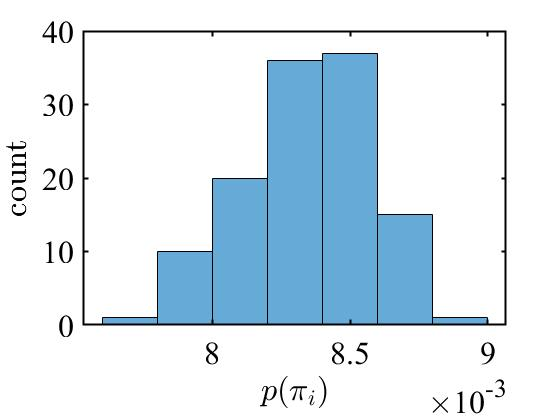
\includegraphics[width=.4\textwidth]{kadai3_histo.jpg}
\end{center}
\caption{課題3のヒストグラム(生成数は$100000$)}%図名
\label{fig:kadai3_3}
\end{figure}

%チェビシェフの不等式の置き換えの大数の弱法則から,
%\begin{equation}
%P(|\overline{X}_n-\mu|\ge \epsilon) \le \dfrac{\sigma^2}{n \epsilon^2}
%\end{equation}
%となる.ここでの$\overline{X}_n$はサンプルデータ$n$までの平均値(標本),$\mu$は理論的に考えられる平均値,$\epsilon$は許容誤差の大きさ,$\sigma$は標本データの分散である.




%$A^1$\cite{aaa}%参考文献




%\begin{itemize}
%\item アイテムコード1
%\item アイテムコード2
%\item アイテムコード3
%\item アイテムコード4
%\item アイテムコード5
%\end{itemize}


%\begin{figure}[H]%[h]は記述したところ。[t]はそのページの上端。[t]はそのページの下端、[p]はページいっぱい
%\begin{center}
%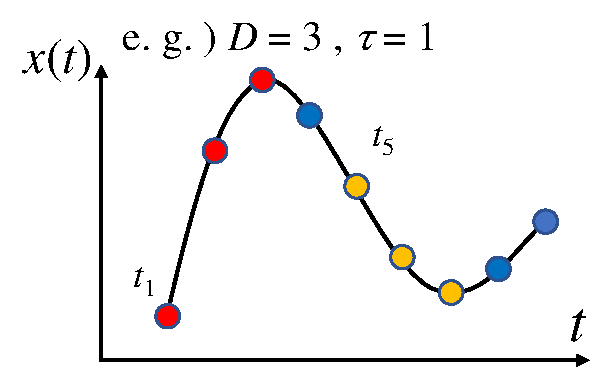
\includegraphics[width=.4\textwidth]{crop_PE1ver2.pdf} 
%\end{center}
%\caption{時系列$ x(t) $}%図名
%\label{fig:PE1}%fig図tb表
%\end{figure}

%\begin{eqnarray}
%\left\{%%{を作る
%\begin{array}{l}%l,llでは、lのときすべて{}の中の式のとき、{}の中にないものがあるならこっち
%\end{array}
%\right.
%\end{eqnarray} 


\begin{thebibliography}{9999}%参考文献
\bibitem{lo}%参考文献citeするぞ
ローレンツ方程式,\url{http://www.isc.meiji.ac.jp/~random/lecture/2015-comp2/Lorentz_equ.html}
\bibitem{re}
カオス・フラクタル\ 講義ノート\ \#8,\url{https://ocw.hokudai.ac.jp/wp-content/uploads/2016/01/ChaosFractal-2011-Note-08.pdf}
\bibitem{wgn}%参考文献citeするぞ
ホワイトガウスノイズサンプルの生成-MATLAD wgn,\url{https://jp.mathworks.com/help/comm/ref/wgn.html}
\bibitem{logi}
ロジスティック写像の時系列 - 工学院大学,\url{https://brain.cc.kogakuin.ac.jp/~kanamaru/Chaos/Logits/}
\bibitem{mutual}
相互情報量の意味とエントロピーとの関係 | 高校数学の美しい物語,\url{https://mathtrain.jp/mutualinfo}
\bibitem{net}
複雑ネットワーク:統計物理学の視点,\url{http://mercury.yukawa.kyoto-u.ac.jp/~bussei.kenkyu/pdf/03/1/9999-031210.pdf}
\end{thebibliography}

%\newpage



\end{document}